\documentclass[11pt,letterpaper]{report}
\usepackage[margin=1in]{geometry}
\usepackage[utf8]{inputenc}
\usepackage[T1]{fontenc}
\usepackage{helvet}
\renewcommand{\familydefault}{\sfdefault}
\linespread{1.5}
\usepackage[spanish,es-nodecimaldot]{babel}
\usepackage{titlesec}
\usepackage[hidelinks]{hyperref}
\usepackage[skip=0pt plus8pt, indent=1.25cm]{parskip}

% Formato de tabla y de título de tabla
\usepackage{graphicx}
\usepackage{caption}
\captionsetup[table]{skip=0pt,singlelinecheck=off}

\usepackage{pdfpages}
% Formatos de títulos
\titleformat{\chapter}[block]{\normalfont\fontsize{12pt}{12pt}\bfseries}{SECCIÓN \ \thechapter.}{0.6em}{\centering\MakeUppercase}
\titlespacing*{\chapter}{0em}{*3}{*2}
\titleformat{\section}[block]{\normalfont\fontsize{12pt}{12pt}\bfseries}{\thesection}{0.6em}{}
\titlespacing*{\section}{0em}{*2}{*1.2}
\titleformat{\subsection}[block]{\normalfont\bfseries\itshape}{\thesubsection}{0.6em}{}
\titlespacing*{\subsection}{4em}{*1}{*0.6}

% Formato de citación
\usepackage{csquotes}
\usepackage[backend=biber, style=vancouver]{biblatex}
\DeclareFieldFormat*{url}{\bibstring{urlfrom}: \url{#1}}
\DeclareFieldFormat{urldate}{[\bibstring{urlseen}: \space#1]}
\addbibresource{mydocument.bib}

\DefineBibliographyStrings{spanish}{
	urlfrom = {Disponible en},
	urlseen = {Accedido},
}

% Formato de numeración
\renewcommand*{\theenumi}{\thesection.\arabic{enumi}}
\renewcommand*{\theenumii}{\theenumi.\arabic{enumii}}

% Cosas generales
\title{Factores de riesgo en el neurodesarrollo infantil}
\author{Soto Consuegra, Josué Daniel \and López Castillo, Sarah Ivón \and
Ixquiac Vásquez, Etelvina Del Rosario \and Guzmán Pérez, Mariana Del Rosario
\and Mazariegos Manrique, Sonia María}
\newcommand{\tiempito}{durante mayo de 2025}
\newcommand{\muestradeseada}{1,701}
\newcommand{\asq}{“Cuestionario Edades y Etapas 3”}

\begin{document}
%	\chapter*{Dedicatoria}
%	\chapter*{Agradecimiento}
%	\chapter*{Resumen}
	\tableofcontents
%	\chapter{Introducción}
	\chapter{Planteamiento del problema}
\section{Descripción del problema}
\section{Delimitación del problema}
	\begin{enumerate}
		\item Ámbito geográfico:
		\item Ámbito institucional:
		\item Ámbito poblacional:
		\item Ámbito temporal:
		\item Ámbito temático:
	\end{enumerate}\
\section{Preguntas de investigación}
	\begin{enumerate}
		\item ¿Qué patrones específicos de riesgo en los dominios del
			neurodesarrollo pueden identificarse mediante el Cuestionario
			Edades y Etapas 3 en niños menores de 5 años que asisten a
			servicios de atención primaria en Quetzaltenango?
		\item ¿Cuál es la asociación entre factores socioeconómicos,
			demográficos, familiares y antecedentes perinatales con el riesgo
			de retraso en cada uno de los cinco dominios del neurodesarrollo
			evaluados mediante el ASQ-3 en niños menores de 5 años en
			Quetzaltenango?
		\item ¿En qué medida el acceso a servicios de atención primaria durante
			los períodos prenatal y postnatal modifica la asociación entre
			factores de riesgo socioeconómicos y el desarrollo infantil
			temprano en los distintos dominios evaluados por el Cuestionario
			Edades y Etapas 3?
	\end{enumerate}

	\chapter{Objetivos}
\section{Objetivo general}
	\begin{enumerate}
		\item Establecer la asociación entre factores sociodemográficos,
		económicos, familiares y médicos con el riesgo en el neurodesarrollo en
		niños menores de 5 años que asisten a servicios de atención primaria en
		el distrito de Quetzaltenango, mediante evaluaciones con el \asq\
		durante 2025.
	\end{enumerate}
\section{Objetivos específicos}
	\begin{enumerate}
		\item Clasificar los resultados del \asq\ según grupos de edad para
		detectar patrones específicos de riesgo en los dominios del
		neurodesarrollo.
		
		\item Evaluar la asociación entre factores socioeconómicos,
		demográficos, ambientales y antecedentes perinatales y el riesgo de
		retraso en el neurodesarrollo utilizando el \asq.
		
		\item Analizar la relación entre acceso a servicios de atención
		primaria durante el periodo prenatal y postnatal con la presencia de
		riesgo de retraso en el neurodesarrollo.
	\end{enumerate}

	\chapter{Justificación}
Los trastornos del desarrollo, también conocidos como retrasos del desarrollo,
constituyen un grupo heterogéneo de condiciones que afectan el aprendizaje, el
lenguaje, el comportamiento o las habilidades motoras.
\cite{cdcDevelopmentalDisability} Estos retrasos se identifican cuando un niño
no alcanza los hitos de desarrollo esperados en comparación con sus pares de la
misma población \cite{DevelopmentalSurveillance}. Por ello es importante
destacar que el retraso en el desarrollo no es un diagnóstico en sí mismo, sino
un término descriptivo utilizado en la práctica clínica para indicar un
fenotipo amplio que requiere una evaluación más detallada para determinar las
áreas específicas de desarrollo afectadas. Hay tres tipos de retraso en el
desarrollo basado en el número de dominios involucrados: 1) Retraso aislado en
el desarrollo: involucra un solo dominio; 2) Múltiples retrasos en el
desarrollo: 2 o más dominios o líneas de desarrollo afectados; y, 3) Retraso
global en el desarrollo: retraso significativo en la mayoría de los dominios de
desarrollo. \cite{Bellman2013} Aunque la etiología de la mayoría de los
retrasos en el desarrollo es idiopática, cuando se identifica, puede incluir
factores genéticos, ambientales y/o psicosociales. \cite{DevelopmentalDelay}

En Guatemala, según el informe de la línea de base de la Gran Cruzada Nacional
por la Nutrición 2021/2022 de la Secretaría de Seguridad Alimentaria y
Nutricional, solo el 1.9\% de las madres de niños entre 2 y 5 años reportaron
que sus hijos habían asistido alguna vez a un programa de primera infancia, y
apenas el 0.6\% asiste actualmente a un Centro Comunitario de Desarrollo
Infantil Temprano. Más preocupante aún, solo el 49.8\% de los niños de 24 a 59
meses se encuentran en el camino adecuado de desarrollo, salud, aprendizaje y
bienestar psicosocial. \cite{SESAN2022}

A nivel global, según un reporte de UNICEF en 2023, se estima que 250 millones
de niños menores de 5 años están en riesgo de no alcanzar su potencial de
desarrollo. Aproximadamente 200 millones de niños menores de 5 años no están
creciendo, no presentan un adecuado desarrollo global, debido a la desnutrición
en la primera infancia. Además, más de 2 de cada 5 niños entre 3 y 4 años no
reciben la estimulación temprana ni el cuidado parental adecuados. Como
resultado de estas y otras amenazas, el 29\% de los niños de 3 a 5 años no
están logrando un desarrollo apropiado. \cite{UNICEF2023}

El neurodesarrollo infantil es un proceso complejo y dinámico que sienta las
bases para el futuro cognitivo, emocional y social de los individuos. En
Quetzaltenango, Guatemala, existe una brecha significativa en la investigación
sobre los factores que influyen en el desarrollo neurológico de los niños
menores de 5 años. Esta carencia de datos locales específicos obstaculizan la
implementación de intervenciones efectivas y políticas públicas adecuadas.

Para llevar a cabo este estudio en Quetzaltenango, es necesario un equipo de 5
investigadores debido a la complejidad y el alcance de la muestra, la cual
comprende \muestradeseada\ niños. La distribución del trabajo se detalla a
continuación:

	\begin{itemize}
		\item Carga de trabajo y distribución: Cada investigador estará a cargo
		de evaluar aproximadamente 340 niños, lo cual permite una división
		equitativa para asegurar una atención detallada en cada caso. Esto es
		crucial para mantener la calidad de los datos y la consistencia en la
		recolección de información, aspecto necesario para la validez del
		estudio.
		\item Tiempo estimado de evaluación: Cada evaluación individual tomará
		alrededor de 30 a 50 minutos. Esto representa aproximadamente 1,417
		horas en total o 283 horas por investigador. La presencia de 5
		investigadores optimiza el proceso y asegura que las evaluaciones se
		realicen en el tiempo programado.
		\item Cobertura de múltiples puntos de atención: La investigación se
		llevará a cabo en tres servicios de atención primaria de
		Quetzaltenango: el Centro de Salud de Quetzaltenango, el Puesto de
		Salud de Pacajá y el Puesto de Salud de San José Chiquilajá.
		\item Atención a casos en riesgo: Los niños identificados con riesgo en
		el neurodesarrollo y sus padres o tutores recibirán plan educacional y
		material de apoyo para promover actividades de estimulación temprana en
		casa. El mismo lo llevará a cabo el investigador utilizando
		herramientas recomendadas por UNICEF.
	\end{itemize}

En conclusión, la integración de un equipo de 5 investigadores permite abordar
de manera exhaustiva y precisa los desafíos de la evaluación de neurodesarrollo
en niños menores de 5 años en Quetzaltenango. Los resultados esperados no solo
aportarán evidencia científica local, sino que también promoverán
intervenciones que puedan mejorar el desarrollo integral de los niños,
sensibilizando a las autoridades y profesionales de la salud sobre la
importancia de intervenciones tempranas y costo efectivas en el desarrollo de
la primera infancia.

	\chapter{Marco teórico}
\section{Antecedentes y contextualización del problema de investigación}
En un estudio transversal realizado por Mehner et al. (2019), titulado "La
asociación de la puntuación de riesgo acumulativo con los resultados de ASQ-3
en una región rural empobrecida de Guatemala", se evaluó una muestra de
conveniencia de 148 madres con niños de 12 a 52 meses de edad en una zona
rural de Guatemala. El objetivo principal fue desarrollar una puntuación de
riesgo compuesta por factores fácilmente obtenibles para diseñar intervenciones
e identificar a los niños de alto riesgo que más se beneficiarían de estas.
Se utilizaron encuestas de interacción madre-hijo y \asq\ para evaluar el
desarrollo. Los resultados mostraron que el 58\% de los niños tenían
puntuaciones anormales en $\ge$1 dominio del ASQ-3, y el 35\% en $\ge$2
dominios. Se desarrollaron tres puntuaciones de riesgo: Riesgo Demográfico
Materno (DR), Interacción Madre-Hijo (MCI) y Riesgo Combinado (CR). La
probabilidad de tener $\ge$2 dominios con puntuaciones anormales aumentó
significativamente con un puntaje DR creciente (OR, 1.46 [IC 95\%, 1.15-1.86]
p<0.05) y un puntaje CR creciente (OR, 2.08 [IC 95\%, 1.41-3.07], p<0.05). Los
autores concluyeron que un índice de riesgo acumulativo combinado de factores
demográficos e interacciones madre-hijo parece ser una herramienta útil para
predecir qué niños tienen puntuaciones anormales en múltiples dominios del
desarrollo. \cite{CMehner2019}

En el contexto específico de Guatemala, un análisis del informe de la  línea de
base de la Gran Cruzada Nacional por la Nutrición 2021/2022 revela  datos
preocupantes: la cobertura de programas de primera infancia es extremadamente
limitada, con apenas un 1.9\% de niños entre 2 y 5 años que han asistido alguna
vez a estos programas. Más alarmante aún es que solo el 49.8\% de los niños
guatemaltecos entre 24 y 59 meses muestran un desarrollo adecuado  en las
dimensiones de salud, aprendizaje y bienestar psicosocial \cite{SESAN2022}.
Estos datos son consistentes con las observaciones de Mehner et al.
\cite{CMehner2019} en zonas rurales de Guatemala, donde encontraron que el 58\%
de los niños evaluados presentaban puntuaciones anormales en al menos un
dominio del ASQ-3.

En una revisión sistemática y meta-análisis realizada por Wondmagegn et al.
(2024), titulada "Prevalencia y determinantes del retraso del desarrollo entre
los niños en países de ingresos bajos y medios: una revisión sistemática y un
metanálisis", se analizaron 21 estudios primarios publicados entre 2010 y
2024, involucrando a un total de 54,067 niños en países de ingresos bajos y
medios. El objetivo principal fue evaluar la prevalencia combinada del retraso
del desarrollo confirmado y sus determinantes entre los niños en estos países.
Los resultados mostraron una prevalencia combinada de retraso del desarrollo
del 18.83\% (IC 95\%: 15.53-22.12\%). En el análisis de subgrupos, se observó
una alta prevalencia de retraso del desarrollo [26.69\% (IC 95\%: 15.78-37.60)]
en estudios realizados en África. Los determinantes significativos del retraso
del desarrollo fueron la educación materna [OR: 3.04; IC 95\% (2.05, 4.52)] y
el bajo peso al nacer [OR: 3.61; IC 95\% (1.72, 7.57)]. Los autores concluyeron
que la prevalencia combinada de retraso del desarrollo en países de ingresos
bajos y medios era alta en comparación con los países de altos ingresos,
especialmente en África, y que el nivel educativo materno y el peso al nacer
estaban significativamente asociados con los retrasos del desarrollo.
\cite{Wondmagegn2024}

En un estudio transversal comunitario realizado en áreas urbanas de Etiopía por
Delbiso et al. (2024), titulado "Desarrollo de la primera infancia y estado
nutricional en la Etiopía urbana", se evaluaron 627 pares de madres e hijos de
12-36 meses de edad entre julio y septiembre de 2022. El desarrollo infantil
temprano (DIT) se evaluó utilizando el \asq, mientras que el estado nutricional
se determinó mediante mediciones antropométricas. Los resultados mostraron que
los retrasos en los dominios del DIT eran comunes, especialmente en el dominio
motor fino (41.9\%). Más de la mitad de los niños (52.8\%) presentaban retraso
en el crecimiento. Se encontró que el retraso en el crecimiento y el bajo peso
estaban asociados con retrasos en el DIT, mientras que la desnutrición aguda no
lo estaba. Los niños con retraso en el crecimiento tenían más probabilidades de
tener peores retrasos en el DIT en los dominios motor fino (OR = 1.54; IC 95\%:
1.11-2.15), motor grueso (OR = 1.47;IC 95\%: 1.05-2.04) y resolución de
problemas (OR = 1.41; IC 95\%: 1.02-1.96) en comparación con los niños sin
retraso en el crecimiento. De manera similar, los niños con bajo peso tenían
más probabilidades de tener peores retrasos en el DIT en los dominios motor
grueso (OR = 1.91; IC 95\%: 1.20-3.04) y motor fino (OR = 1.90; IC 95\%:
1.15-3.15) en comparación con los niños de peso normal. \cite{Delbiso2024}

Domek et al. (2023) realizaron un estudio piloto para evaluar los efectos a
largo plazo de una intervención simple con títeres de dedo para promover el
desarrollo infantil temprano en el ámbito de atención primaria. La muestra
incluyó 172 niños de familias principalmente de bajos ingresos, divididos en
cohortes de intervención temprana (2 meses) y tardía (6 o 12 meses). Se utilizó
el \asq\ para evaluar el desarrollo infantil hasta los 36 meses. Los resultados
mostraron que la intervención temprana se asoció con mejores trayectorias de
desarrollo socioemocional en comparación con
la intervención tardía (diferencia en pendiente de 0.12, p=0.018). También se
observaron diferencias que se acercaron a la significancia estadística en
comunicación (p=0.056) y en la puntuación combinada no motora (p=0.052). No se
encontraron diferencias significativas en los dominios de resolución de
problemas, motricidad gruesa y fina. Los autores concluyeron que la
intervención con títeres de dedo puede proporcionar una forma simple, de bajo
costo y escalable de fomentar interacciones cuidador-infante que promuevan el
desarrollo del lenguaje y socioemocional, especialmente cuando se proporciona
en la infancia temprana. Este estudio destaca la importancia de las
intervenciones tempranas en atención primaria y su potencial impacto en el
desarrollo infantil a largo plazo. \cite{Domek2023}

En un estudio transversal, descriptivo y exploratorio realizado por Ramos y
Della Barba (2021), titulado Cuestionarios de edades y etapas de Brasil en el
seguimiento del desarrollo en la primera infancia, se analizaron 392 niños de 
5 a 50 meses de edad que asistían a 6 Centros de Educación Infantil (CEIs) en
un municipio del interior del estado de São Paulo, Brasil. El objetivo
principal fue delinear el perfil del desarrollo global de los niños utilizando 
el \asq\ edición Brasil (ASQ-BR) y verificar la aplicabilidad
de este instrumento por parte de los maestros preescolares. Los resultados
mostraron que la mayoría de los niños presentaron un desarrollo dentro de lo 
esperado, con los mejores desempeños en los dominios de Motricidad Gruesa
(79.44\%), Comunicación (72.34\%) y Resolución de Problemas (69.54\%). Sin
embargo, se observó una incidencia significativa de riesgo en los dominios
Personal-Social (22.08\%) y Motricidad Fina (19.03\%). En el análisis por sexo,
las niñas obtuvieron puntuaciones significativamente más altas que los niños en
los dominios de Motricidad Fina y Personal-Social. Los autores concluyeron que
el ASQ-BR se presenta como un instrumento potencial para el cribado del
desarrollo infantil en guarderías y preescolares, permitiendo a los
profesionales reflexionar sobre su propia práctica y atender mejor las
necesidades individuales de los niños. \cite{RAMOS2021}

Oumer et al. (2022), titulado “El retardo de crecimiento y bajo peso, pero no
la desnutrición aguda, están asociados con el retraso en el desarrollo
infantil en el suroeste de Etiopía”, se analizaron 507 pares de madres e hijos
en el Suroeste de Etiopía. El objetivo principal fue identificar la relación
entre diferentes formas de malnutrición y el retraso en el desarrollo infantil
entre niños de 12 a 59 meses de edad. Los resultados mostraron una prevalencia
de retraso en el desarrollo del 29.4\% (IC 95\%: 25.4-33.4\%). En el análisis
de subgrupos, se observaron retrasos en el desarrollo de habilidades motoras
gruesas (17.2\%), comunicación (16.8\%), resolución de problemas (13.4\%),
habilidades personales-sociales (10.8\%) y motricidad fina (10.1\%).
Los determinantes significativos del retraso en el desarrollo fueron el trabajo
materno fuera del hogar [AOR: 2.9; IC 95\% (1.8, 4.8)], el nacimiento prematuro
[AOR: 3.2; IC 95\% (1.4, 7.0)], la iniciación temprana de la alimentación
complementaria [AOR: 2.5; IC 95\% (1.37, 4.6)], el retraso en el crecimiento
[AOR: 3.0; IC 95\% (1.9, 4.7)], el bajo peso [AOR: 2.3; IC 95\% (1.1, 4.7)] y
una baja puntuación de diversidad dietética [AOR: 3.1; IC 95\% (1.3, 7.5)].
Los autores concluyeron que el retraso en el desarrollo infantil es un problema
de salud pública en la región y está fuertemente asociado con la desnutrición
crónica, el bajo peso, el consumo de una dieta poco diversificada y prácticas
subóptimas de alimentación infantil.
\cite{Oumer2022}

En el distrito de Quetzaltenango, Guatemala, la vulnerabilidad económica, el
acceso limitado a servicios de salud y los factores nutricionales representan
un riesgo significativo para el neurodesarrollo infantil. Al igual que en otros
países de ingresos bajos y medios, las condiciones adversas en esta región
pueden influir negativamente en los hitos del desarrollo infantil temprano.

Esta problemática local se enmarca en un contexto global igualmente 
preocupante. Según UNICEF\cite{UNICEF2023}, aproximadamente 250 millones de 
niños menores de 5 años a nivel mundial están en riesgo de no alcanzar su 
potencial de desarrollo, con cerca de 200 millones afectados por desnutrición 
en la primera infancia. Particularmente relevante para nuestro estudio es que 
más de 2 de cada 5 niños entre 3 y 4 años no reciben la estimulación temprana 
ni el cuidado parental adecuados, factores que Domek et al.\cite{Domek2023} 
identificaron como críticos para el desarrollo del lenguaje y socioemocional. 

La unión de los datos nacionales con los hallazgos globales subraya la 
necesidad de investigaciones específicas en contextos como Quetzaltenango, 
donde factores socioeconómicos, nutricionales y de acceso a servicios de salud 
pueden influir significativamente en los patrones de desarrollo infantil.

\section{Neurodesarrollo}
El neurodesarrollo es un proceso dinámico de interacción entre el niño y el 
entorno que lo rodea, necesario para el aprendizaje y la productividad. Abarca
diversos dominios neurológicos esenciales: sensorial, motor, lingüistico,
visuo-espacial, intelectual, memoria, cognición social y función ejecutiva.
\cite{Nelson46}

El desarrollo del cerebro humano es un proceso prolongado que comienza en la 
tercera semana gestacional con la diferenciación de células progenitoras 
neurales y se extiende al menos hasta la adolescencia tardía, posiblemente 
durante toda la vida. Los procesos que contribuyen al desarrollo cerebral van 
desde eventos moleculares de expresión genética hasta influencias ambientales. 
Es fundamental entender que estos diferentes niveles y tipos de procesos 
interactúan para sustentar la serie continua de eventos que definen el 
desarrollo cerebral.
\cite{Stiles2010}

Tanto la expresión genética como los estímulos ambientales son esenciales para 
el desarrollo cerebral normal, y la alteración de cualquiera de estos factores 
puede modificar fundamentalmente los resultados neurales. Sin embargo, ni los 
genes ni los estímulos son determinantes absolutos del resultado final. El
desarrollo cerebral se caracteriza más apropiadamente como una serie compleja
de procesos dinámicos y adaptativos que operan a lo largo del desarrollo para
promover la diferenciación de nuevas estructuras y funciones neurales.
\cite{Stiles2010}

Los primeros años de vida se caracterizan por un desarrollo acelerado, durante
el cual numerosas estructuras neuronales se construyen y organizan. En esta
etapa crucial, las experiencias tienen mayor capacidad de penetrar
profundamente y modelar el desarrollo futuro del niño. Procesos como la poda
neuronal o sináptica y la metilación del ADN permiten que las experiencias
modifiquen el cerebro en desarrollo, por lo que interacciones biológicas y del
entorno son importantes en el neurodesarrollo. \cite{Feldman2}

\section{Procesos biológicos del desarrollo cerebral}
El cerebro humano evoluciona a partir de un grupo limitado de células
embrionarias hasta convertirse en el sistema orgánico más complejo, todo ello
durante los escasos 280 días que comprende la gestación humana. Lo que 
distingue principalmente el desarrollo fetal humano del de otras especies es 
precisamente el cerebro, con su masiva corteza prefrontal y su extraordinaria 
capacidad para investigar y reflexionar sobre su propia naturaleza y 
funcionamiento. \cite{Polin124}

Durante el neurodesarrollo, los eventos genéticos y epigenéticos se entrelazan 
siguiendo una regulación estricta, tanto temporal como espacial, transformando
un delgado disco de neuroepitelio indiferenciado en un sofisticado sistema de
múltiples capas. \cite{Polin124}

El proceso de desarrollo cerebral, genéticamente predeterminado, comprende
siete fases claramente definidas que se despliegan a lo largo de un extenso
período evolutivo. \cite{Kolb7} Mientras algunas de estas fases están
circunscritas a períodos específicos, otras mantienen su actividad durante
intervalos temporales más prolongados. Las características de estas fases se
sintetizan en el cuadro \ref{tab:fases-desarrollo-cerebral}.

\begin{table}[htbp]
\caption{Siete fases del desarrollo cerebral}
\label{tab:fases-desarrollo-cerebral}
\resizebox{\textwidth}{!}{%
\begin{tabular}{ll}
\hline
\multicolumn{1}{c}{\textbf{Fase del desarrollo}} & \multicolumn{1}{c}{\textbf{Proceso}} \\ \hline
1. Nacimiento celular & Origen de las neuronas y la glia \\
2. Migración celular & Movimiento de las células a su posición funcional \\
3. Diferenciación celular & Las células precursoras se transforman en un tipo de célula especializada \\
4. Maduración celular & Crecimiento de dendritas y axones \\
5. Sinaptogénesis & Formación de sitios de comunicación de célula a célula \\
6. Muerte celular y poda sináptica & Muerte celular programada y desmantelamiento de circuitos no usados \\
7. Mielinización & Formación de la vaina de mielina que aumenta la velocidad de neurotransmisión \\ \hline \hline
\footnotesize Fuente: Kolb, B y Whishaw, I y Campbell T. \cite{Kolb7}
\end{tabular}%
}
\end{table}

\subsection{Desarrollo cerebral en el período embrionario}
\subsubsection{Gastrulación: establecimiento de las capas germinales primordiales}
Uno de los primeros pasos cruciales en el desarrollo cerebral ocurre durante la
tercer semana de gestación, cuando la masa celular interna bilaminar, compuesta
por el epiblasto y el hipoblasto, experimenta el proceso de gastrulación para
formar las tres capas germinales embrionarias fundamentales: endodermo,
mesodermo y ectodermo. \cite{Polin124}

Este proceso se inicia con la aparición de la línea primitiva en la superficie
del epiblasto y la definición del polo cefálico, denominado nodo primitivo. La
formación de la línea primitiva está principalmente controlada por la
activación de la vía de señalización Wnt. \cite{MooreEmbryo4}

Durante la gastrulación, el epiblasto adquiere la capacidad de migrar hacia la
línea primitiva mediante el proceso de transformación epitelio-mesenquimal. La
disminución de la adhesión celular permite que las células migratorias del
epiblasto se invaginen en la región del nodo y la línea primitiva, deslaminen
y desplacen a las células del hipoblasto para formar el endodermo y el
mesodermo. Las células restantes del epiblasto se diferencian en ectodermo. El
mesodermo dorsal da origen a la notocorda, estructura que posteriormente induce
al ectodermo suprayacente a engrosarse y formar la placa neural, dando lugar al
neuroectodermo. Este momento marca el final de la gastrulación y el inicio de
la neurulación. \cite{Polin124}

La gastrulación también establece visiblemente los ejes primarios del embrión y
del sistema nervioso: lateral, anteroposterior y dorsoventral. Para el día
embrionario 20, las tres capas germinales (endodermo, mesodermo y ectodermo)
están completamente formadas, siendo el ectodermo la capa que dará origen tanto
a la piel como al sistema nervioso central. \cite{Polin124}

\subsubsection{Neurulación: formación del tubo neural}
La neurulación es el proceso mediante el cual se forma el tubo neural a partir
del plegamiento de la placa neural epitelial. En humanos, este proceso ocurre
en dos fases distintas: la neurulación primaria, durante las semanas 3 y 4 de
gestación, que conduce al desarrollo del cerebro y la médula espinal, y la
neurulación secundaria, durante las semanas 5 y 6, con la formación de la
porción inferior de la médula espinal sacra y coccígea. \cite{Polin124}

La placa neural se forma aproximadamente el día embrionario 21 y para el día 22
el surco neural se hace evidente. La fusión del surco neural comienza el día 23
para formar el tubo neural, cerrándose primero la sección central. La porción
rostral del tubo neural, habitada por las primeras células migratorias, se
convertirá en el cerebro, mientras que la porción caudal, que recibe células
migratorias posteriores, formará la médula espinal. Las regiones rostral y
caudal del tubo neural son las últimas en cerrarse. \cite{Gibb2018}

Durante la neurulación, la población de células madre neurales experimenta una
rápida expansión mediante división celular simétrica de las células
neuroepiteliales (CNE). Las CNE generadas en este periodo están influenciadas
por la expresión de las moléculas de señalización Emx2 y Pax6, que producen
progenitores destinados a regiones cerebrales específicas. \cite{Gibb2018}

Para satisfacer la demanda de neuronas que poblarán el cerebro, alrededor del
día 25, las CNE comienzan a dividirse de manera simétrica, produciendo dos
CNE con cada división, proceso que continúa hasta aproximadamente el día 42.
Poco antes del inicio de la neurogénesis, estas células pierden sus uniones
estrechas, comienzan a expresar genes gliales e inician su transformación en
células gliales radiales. \cite{Stiles2010}

\subsubsection{Formación de vesículas cerebrales primarias y secundarias}
Al finalizar la neurulación, el embrión mide entre 3 y 5 mm de longitud, y para
el final de la octava semana gestacional alcanza entre 27 y 31 mm, un
incremento de diez veces su tamaño. Durante este periodo, la forma del sistema
nervioso primitivo cambia dramáticamente. \cite{Stiles2010}

Justo antes del cierre completo del tubo neural, el extremo anterior del tubo
comienza a expandirse formando las tres vesículas cerebrales primarias: el
prosencéfalo (la vesícula más anterior, precursora del cerebro anterior), el
mesencéfalo (vesícula media, precursora de las estructuras del cerebro medio) y
el rombencéfalo (vesícula posterior, que se desarrollará como cerebro
posterior). \cite{Stiles2010}

Estos tres segmentos se subdividen posteriormente y, al final del periodo
embrionario, están presentes las cinco vesículas cerebrales secundarias. El
prosencéfalo se divide en telencéfalo y diencéfalo, mientras que el
rombencéfalo se divide en metencéfalo y mielencéfalo. El mesencéfalo permanece
sin subdividirse. Estas cinco subdivisiones se alinean a lo largo del eje
rostro-caudal del embrión y establecen la organización primaria del sistema
nervioso central. \cite{Stiles2010}

\subsection{Desarrollo cerebral en el período fetal}
Los eventos embrionarios de las primeras seis semanas de desarrollo establecen
el patrón tridimensional del cerebro y la médula espinal, determinando el
destino de las primeras células neurales. Las etapas posteriores del desarrollo
se caracterizan por una proliferación y diferenciación masiva de neuronas y
células gliales, seguidas por la migración y organización de la corteza
cerebral y cerebelosa, el crecimiento dendrítico, la sinaptogénesis y,
finalmente, la formación de vainas de mielina alrededor de las neuronas.
\cite{Polin124}

Durante esta fase del desarrollo cerebral, el cerebro previamente liso adquiere
el patrón de plegamiento con giros y surcos típicamente observados en el
cerebro maduro. Este proceso de desarrollo no consiste en fases temporalmente
separadas, sino en una superposición continua de proliferación, migración y
organización neuronal. \cite{Gibb2018}

\subsubsection{Fase 1 - Nacimiento celular}
Todas las neuronas y células gliales derivan de centros proliferativos
especializados cercanos a la superficie pial: la zona ventricular, la zona
subventricular y, como se ha descrito más recientemente, la zona subventricular
externa. El crecimiento cerebral se caracteriza por la proliferación neuronal
entre las semanas 8 y 15 del desarrollo, y posteriormente por la generación de
glía radial que cambia a una multiplicación principalmente glial a mediados del
segundo trimestre, extendiéndose hasta la vida posnatal. Cierta proliferación
neuronal ocurre más tarde en la gestación, principalmente en la capa granular
externa del cerebelo y en la zona subventricular. \cite{Polin124} 

El primordio cortical está compuesto por células madre neurales pluripotentes
en división y células progenitoras neurales más restrictivas que colectivamente
forman la zona ventricular. Estas células neurales se dividen mediante el
proceso único de movimiento nuclear intercinético. A medida que el núcleo se
mueve en consonancia con el ciclo celular, el ambiente a lo largo del eje
apical-basal expone los núcleos a diferentes señales, proliferativas versus
neurogénicas. Estos eventos proliferativos tempranos aumentan dramáticamente el
grosor y la superficie de la zona ventricular, particularmente en el
prosencéfalo. \cite{Polin124}

Derivadas de la zona ventricular, las células de la glía radial mantienen mayor
pluripotencia y son capaces de producir tanto neuronas como células gliales
(astrocitos y oligodendrocitos). Las células gliales radiales son células no
neuronales elongadas que cumplen dos funciones: actúan como andamio guía para
la posterior migración de neuronas y como progenitores neurogénicos y gliales.
\cite{Polin124}

\subsubsection{Fase 2 - Migración celular}
Entre las semanas 12 y 20 de gestación, millones de neuronas postmitóticas se
desplazan desde sus sitios de origen en la zona ventricular y la zona
subventricular hacia la corteza en desarrollo y los núcleos profundos, donde
residirán durante toda la vida, ocupando posiciones específicas para formar la
corteza de seis capas, observable a las 28 semanas de gestación. El momento y
la dirección de estas múltiples migraciones simultáneas están estrictamente
regulados, y los trastornos de este proceso son poco comunes.
\cite{Polin124}

Después de que las células se generan en la zona ventricular o subventricular,
migran de manera radial a lo largo de las células gliales radiales. Las células
que forman las capas más profundas de la corteza cerebral salen primero. 
\cite{Polin124}

\subsubsection{Fase 3 - Diferenciación celular}
Las especializaciones del cerebro humano surgen durante etapas concretas del
neurodesarrollo, un proceso controlado espacial y temporalmente cuya
ontogenia es generalmente compartida entre los mamíferos. La diferenciación
neuronal no constituye un evento aislado, sino un proceso continuo que comienza
con células precursoras, continúa a través de la generación, migración e
integración de neuronas recién formadas en circuitos específicos, y prosigue
durante un prolongado período de maduración neuronal funcional.
\cite{Lindhout2024}

El neurodesarrollo se inicia con la proliferación de células neuroepiteliales
que se transforman en diferentes poblaciones de progenitores neurales. Estos
progenitores dan origen a diversos subtipos neuronales que migran hacia
regiones cerebrales específicas, estableciendo las bases estructurales y
funcionales del cerebro en formación. \cite{Lindhout2024}

En la corteza cerebral, los primeros progenitores que aparecen son la glía
radial apical, que continúan expandiéndose y produciendo tipos adicionales de
progenitores amplificadores, como los progenitores intermedios y la glía radial
basal o externa. Este conjunto de progenitores corticales eventualmente da
origen a las neuronas corticales, que posteriormente migran hacia la superficie
exterior y forman las distintas capas de la corteza en un orden de adentro
hacia afuera. \cite{Lindhout2024}

Los progenitores intermedios producen neuronas, mientras que las células de
glía radial dan origen tanto a neuronas de proyección como a astrocitos. A
medida que se forman capas sucesivas del manto cortical, los progenitores se
vuelven más limitados en los tipos celulares que pueden generar.
\cite{Lindhout2024}

Cuando las células madre multipotentes se diferencian primero en células
progenitoras neurales y posteriormente en neuronas, las alteraciones en la
metilación del ADN, las modificaciones de histonas, la accesibilidad de la
cromatina y la composición de variantes de histonas median cambios específicos
en la transcripción génica asociados con cada etapa del desarrollo.
\cite{Lindhout2024}

\subsubsection{Fase 4 - Maduración celular}
Una vez que las neuronas alcanzan su destino final, extienden dendritas y un
axón en un intento de establecer conexiones con otras células y convertirse en
parte integral de una red de comunicación. Las dendritas recopilan información
de otras neuronas, mientras que el axón proporciona un medio para enviar
información a neuronas ubicadas más adelante en la línea de comunicación.
Muchas dendritas se extienden desde una neurona para recibir información de
células en la red, pero un solo axón transmite la información procesada por la
célula. \cite{Gibb2018}

Para establecer contactos apropiados, el axón posee un cono de crecimiento en
su extremo principal. Este cono de crecimiento es guiado mediante el muestreo
de moléculas trópicas producidas localmente que finalmente ayudan al axón a
encontrar su objetivo previsto. Una vez identificado ese objetivo, se forma una
conexión llamada sinapsis, que proporciona el medio para la comunicación célula
a célula. En el contexto de la sinapsis, el axón se considera el terminal
presináptico y la dendrita, el terminal postsináptico. \cite{Gibb2018}

\subsubsection{Fase 5 - Sinaptogénesis}
El momento de la formación de sinapsis varía a lo largo del cerebro en
desarrollo. Los principios básicos de la sinaptogénesis incluyen la formación
de las sinapsis más tempranas en las zonas marginal y de la subplaca, un
aumento en el número de sinapsis en la placa cortical hasta un pico que excede
el número adulto, y un período posterior de eliminación sináptica. En el
cerebro, las sinapsis se observan inicialmente en neuronas de la subplaca y la
zona marginal. \cite{Polin124}

Inicialmente, las dendritas aparecen como procesos gruesos con algunas 
ramificaciones finas. A medida que avanza el desarrollo, aparece un gran número
y variedad de espinas dendríticas. Posteriormente comienza la eliminación
sináptica, y se pierde una gran proporción de sinapsis. \cite{Polin124}

Los factores que estimulan la formación y el desarrollo de sinapsis en el
cerebro en desarrollo incluyen tanto eventos independientes de la actividad
como eventos dependientes de la actividad que ocurren después del desarrollo de
receptores en neuronas diana y la generación de actividad eléctrica.
\cite{Polin124}

\subsubsection{Fase 6 - Muerte celular y poda sináptica}
La formación del cerebro también depende de procesos degenerativos que
comienzan en el período prenatal. La muerte celular programada o apoptosis se
inicia para reducir el número de células en el cerebro que no han logrado
establecer conexiones útiles o tienen conexiones infrautilizadas.
\cite{Gibb2018}

La muerte celular y la eliminación selectiva de procesos neuronales y sinapsis,
o poda en el desarrollo cerebral, son críticas para el comportamiento posnatal
normal. Típicamente, aproximadamente la mitad de las neuronas en la región
cortical mueren antes de la maduración final. Este proceso de muerte celular
programada, la apoptosis, se inicia y se mantiene por la expresión de genes
específicos. Un aspecto crítico en las fases finales de la secuencia hacia la
muerte celular es la activación de caspasas. \cite{Polin124}

La apoptosis parece ser desencadenada fundamentalmente por la competencia
neuronal por cantidades limitadas de factores tróficos, generados por el
objetivo, la entrada aferente o la glía asociada, permitiendo el emparejamiento
numérico de poblaciones neuronales interconectadas y la eliminación de
proyecciones aberrantes o incorrectas. \cite{Polin124}

\subsection{Desarrollo cerebral en el período postnatal}
Aunque la producción y migración de neuronas son principalmente eventos
prenatales, el desarrollo cerebral continúa de manera significativa después del
nacimiento. La proliferación y migración de progenitores gliales se extiende
durante un período prolongado después del nacimiento, mientras que la
diferenciación y maduración de estas células prosigue a lo largo de toda la
infancia. \cite{Stiles2010}

En el período postnatal, la neurogénesis continúa únicamente en un grado muy
limitado. No obstante, en la zona subventricular, nuevas neuronas siguen
emergiendo y migrando hacia el bulbo olfatorio. Asimismo, se producen neuronas
en el giro dentado del hipocampo, donde migran desde la capa subgranular
solamente hasta la cercana capa granular. Estas formas excepcionales de
neurogénesis parecen continuar durante toda la vida adulta, pero producen solo
un pequeño porcentaje de la población neuronal total.
\cite{Stiles2010}

En contraste con la neurogénesis limitada, la proliferación y migración de
progenitores gliales continúa durante un período prolongado mientras los
oligodendrocitos y astrocitos se diferencian. \cite{Stiles2010}

La sinaptogénesis que comenzó en el período prenatal continúa en el período
postnatal y a lo largo de toda la vida del individuo. La apoptosis continúa
desempeñando un papel fundamental en el desarrollo cerebral durante el período
postnatal. Las sinapsis poco utilizadas son eliminadas en un proceso denominado
poda sináptica, que optimiza los circuitos neuronales para mejorar la
eficiencia funcional. \cite{Gibb2018}

\subsubsection{Fase 7 - Mielinización}
Aunque cierta mielinización ocurre en el período prenatal, este proceso se
intensifica después del nacimiento y continúa hasta bien entrada la tercera
década de vida. El proceso de mielinización predice la maduración de áreas
corticales. Las áreas motoras y sensoriales primarias del cerebro se mielinizan
primero, mientras que las áreas de asociación lo hacen en último lugar.
\cite{Gibb2018}

En el tercer trimestre de gestación, los oligodendrocitos inmaduros desarrollan
extensiones lineales mientras envuelven los axones en preparación para la
mielinización. En el sistema nervioso central, los oligodendrocitos forman
hasta 40 segmentos separados de mielina en múltiples axones, a diferencia del
sistema nervioso periférico, donde las células de Schwann mielinizan axones
individuales. \cite{Polin124}

Este proceso es seguido por la diferenciación hacia el oligodendrocito maduro,
que podría desencadenarse en parte por señales dependientes de la actividad
axonal. Los oligodendrocitos maduros se convierten en la etapa oligodendroglial
predominante en los meses posteriores al nacimiento a término y dan origen a la
mielinización. \cite{Polin124}

Después del inicio de la mielinización, los procesos intracelulares comienzan a
intensificarse para crear la composición rica en lípidos de la mielina. El
colesterol, los fosfolípidos y los glucoesfingolípidos representan el 70\% de
la membrana mielínica. Estas células han desarrollado un sistema altamente
eficaz para mantener la proporción óptima de clases de lípidos en la membrana
estrechamente envuelta para realizar su función aislante durante la conducción
nerviosa. \cite{Polin124}

\section{Modelo biopsicosocial del desarrollo infantil}
La biología influye en el comportamiento y el entorno, y a su vez, el
comportamiento y el entorno influyen en la biología a lo largo del desarrollo.
Los niños están influenciados directa e indirectamente tanto por su contexto
cercano (ej. relaciones con sus cuidadores) como por factores sociales más
amplios (ej. violencia en el vecindario o creencias comunitarias). El
desarrollo infantil es el producto de la acumulación de interacciones y
experiencias cotidianas, así como del contexto comunitario y cultural más
amplio en el que se crían. Si bien los eventos importantes (como cambios en la
estructura familiar) y las circunstancias (como los recursos familiares) son
relevantes para el desarrollo de los niños, también lo son las interacciones
pequeñas que conforman la vida cotidiana. \cite{Feldman3}

Las influencias tempranas, particularmente aquellas que producen niveles
tóxicos de estrés, afectan al individuo a través de su impacto en los sistemas
de respuesta al estrés del cuerpo, el desarrollo cerebral y la modificación de
la expresión genética. Los cambios epigenéticos, como la metilación del ADN y
la acetilación de histonas, pueden estar influenciados por experiencias
tempranas e impactar la expresión genética sin cambiar la secuencia de ADN.
Estos cambios pueden producir efectos duraderos en la salud y el bienestar del
individuo, y pueden transmitirse a generaciones futuras. \cite{Nelson19}

\subsection{Teorías principales}
Las influencias multinivel y transaccionales en el desarrollo infantil han sido
descritas en dos modelos teóricos fundamentales.

\subsubsection{Teoría de Sistemas Ecológicos de Bronfenbrenner}
La teoría de sistemas ecológicos de Urie Bronfenbrenner propone que existen
múltiples niveles de influencia en el desarrollo infantil, desde las relaciones
con los cuidadores hasta sistemas como las escuelas y lugares de trabajo, hasta
eventos en la sociedad más amplia. El microsistema describe las relaciones e
interacciones directas que tienen los niños, como con cuidadores, hermanos y
compañeros. Estas personas influyen directamente en el niño proporcionando
oportunidades para jugar y aprender, y brindando apoyo emocional. El
microsistema también contiene estructuras con las que el niño interactúa, como
la escuela, el vecindario, entornos de cuidado infantil y la familia. Los niños
tanto influyen como son influenciados por estas relaciones y estructuras.
\cite{Feldman3}

El mesosistema describe la interacción entre las estructuras que están en el
microsistema (ej. influencias bidireccionales entre vecindarios y escuelas).
El exosistema consiste en sistemas sociales más grandes que impactan
estructuras en el microsistema (ej. recursos familiares comunitarios u horarios
laborales de los padres). Los niños no interactúan directamente con el
exosistema, pero experimentan el impacto de los cambios en estos sistemas
sociales. El macrosistema es la capa más externa del entorno de un niño y está
definido por valores culturales, costumbres y leyes que influyen en el
funcionamiento de las capas internas. El cronosistema captura la influencia del
tiempo en el desarrollo infantil, reflejando tanto los procesos de desarrollo
que tienen lugar a lo largo del tiempo como la influencia cambiante de los
eventos (ej. un evento traumático) según su duración y la etapa de desarrollo
en la que ocurren. \cite{Feldman3}

\subsubsection{Modelo Transaccional de Sameroff}
El modelo transaccional de Arnold Sameroff se basa en las ideas de
Bronfenbrenner sobre la bidireccionalidad de los efectos en el desarrollo
infantil. Discute los procesos que tienen lugar entre padres e hijos en las
interacciones cotidianas y a lo largo del tiempo. Este modelo surgió de
observaciones que mostraban que muchos riesgos, como el nacimiento prematuro o
complicaciones durante el parto, estaban asociados con problemas de desarrollo
observables solo para algunos niños, con mayor frecuencia aquellos con riesgos
sociales adicionales (ej. bajo nivel socioeconómico). En otras
palabras, los entornos de los niños moderan el efecto de los riesgos
biológicos tempranos en su desarrollo. La naturaleza y la crianza se consideran
inherentemente inseparables; los genes se expresan dependiendo del entorno, y
los padres responden de manera diferente a los niños según las características
biológicas inherentes del niño. \cite{Feldman3}

Las características de un niño impactan la crianza, y la crianza impacta el
desarrollo infantil; estas cascadas bidireccionales de influencias continúan a
lo largo del tiempo durante el desarrollo. Es fundamental entender que los
comportamientos de los padres en respuesta a los niños están impulsados por
sus interpretaciones y el significado que extraen del comportamiento. Por
ejemplo, el manejo ansioso de un padre puede surgir debido a su percepción
sobre las complicaciones del nacimiento del niño; un padre puede desvincularse
de un niño con un temperamento difícil debido al significado que atribuye al
comportamiento inquieto del niño. \cite{Sameroff2009}

\subsubsection{Modelo de Diátesis-Estrés}
Este modelo sugiere que algunos individuos son más vulnerables a los impactos
del estrés que otros. Las diátesis o predisposiciones hereditarias o
constitucionales pueden incluir factores biológicos, genéticos, relacionados
con el temperamento o cognitivos que predisponen a un niño a ser vulnerable a
las influencias del estrés. Los factores estresantes pueden incluir eventos de
vida discretos, estrés crónico o una acumulación de estresores diarios más
menores. En un entorno favorable para el desarrollo, este modelo sugiere que
tanto los individuos resilientes como los vulnerables probablemente se
desarrollarán bien. En un entorno desafiante, los individuos resilientes se
desarrollarían bien, mientras que los vulnerables no. Aquellos que tienen
mayores predisposiciones a la psicopatología pueden verse abrumados por un
estrés ambiental pequeño a moderado, mientras que los individuos con 
predisposiciones más bajas pueden soportar niveles más altos de estrés
ambiental sin efectos aparentes en su funcionamiento. \cite{Feldman3}

\subsubsection{Teoría de Susceptibilidad Diferencial}
Esta teoría postula que los individuos varían en su plasticidad, o su nivel de
susceptibilidad a las influencias ambientales. \cite{Belsky2021} La
susceptibilidad diferencial puede contribuir a resultados positivos y
negativos. Algunos niños, a veces denominados "orquídeas", son muy sensibles a
su entorno. Cuando están en un entorno que apoya ampliamente su desarrollo y
bienestar, prosperan; sin embargo, cuando están en un entorno que no apoya su
desarrollo, tienen dificultades. Otros niños, a veces denominados "dientes de
león", son menos susceptibles a las influencias ambientales y se desarrollarán
más o menos de la misma manera independientemente de cuán favorable sea su
entorno y sus relaciones. Los niños pueden ubicarse en cualquier punto del
espectro entre estos dos extremos. Este grado de plasticidad se ha vinculado a
diferencias en marcadores genéticos, incluidos 5-HTTLPR, DRD4 y BDNF.
\cite{Belsky2021} La susceptibilidad de un niño puede diferir según las
influencias ambientales específicas y el resultado específico que se esté
considerando. \cite{Feldman3}

\subsection{Relaciones cuidador-niño}
Los cuidadores primarios impactan la biología de un niño a través de sus
interacciones con él. Las interacciones que un niño tiene con el cuidador, o
respaldadas por él, dejan una marca duradera en el genoma del niño y en la
estructura cerebral. A través de la poda neuronal, las conexiones neuronales
del niño se refuerzan o se eliminan según sus experiencias. Los efectos
epigenéticos, incluidos los relacionados con la experiencia del cuidado
temprano, también están activos durante este período de desarrollo.
\cite{Roth2011}

La influencia del entorno de crianza domina la mayoría de los modelos actuales
de desarrollo. Los bebés en hospitales y orfanatos, carentes de oportunidades
para el apego, tienen déficits de desarrollo severos. El apego se refiere a
una tendencia determinada biológicamente de un niño pequeño a buscar
proximidad con sus padres durante momentos de estrés y a la relación que
permite a los niños con apego seguro utilizar a sus padres para restablecer una
sensación de bienestar después de una experiencia estresante. El apego inseguro
puede ser predictivo de problemas de comportamiento y aprendizaje posteriores.
\cite{Nelson19}

En todas las etapas del desarrollo, los niños progresan de manera óptima
cuando tienen cuidadores adultos que prestan atención a sus señales verbales y
no verbales y responden en consecuencia. En la primera infancia, esta
capacidad de respuesta contingente a signos de sobreestimulación o baja
estimulación ayuda a mantener a los infantes en un estado de alerta tranquila y
fomenta la autorregulación autonómica. Las respuestas contingentes consistentes
(refuerzo dependiente del comportamiento del otro) a gestos no verbales crean
la base para la atención compartida y la reciprocidad que son críticas para el
desarrollo posterior del lenguaje y social. \cite{Nelson19}

Los cuidadores sirven como guía para el desarrollo cognitivo, social,
conductual, emocional y físico de los infantes. Los niños pequeños no son
capaces de autorregularse desde el punto de vista del desarrollo, por lo que
los cuidadores desempeñan un papel crucial al ayudarlos a lidiar con los
afectos negativos, leyendo sus señales, anticipando transiciones, redirigiendo
su atención y respondiendo rápidamente a sus necesidades. A medida que los
niños adquieren experiencia con sus cuidadores corregulando sus emociones,
comienzan a internalizar estas estrategias de regulación y gradualmente
desarrollan la capacidad de regularse de forma independiente. La crianza
sensible y receptiva promueve resultados positivos en los niños en dominios que
incluyen el apego, el desarrollo cognitivo, las habilidades sociales y la
regulación emocional. Un cuidador sensible y receptivo está sintonizado con los
sentimientos y necesidades del niño, y responde con prontitud con acciones que
están en sintonía con los sentimientos y necesidades del niño durante las
actividades cotidianas (ej. alimentación, juego, baño, cambio de pañales o
ropa).
\cite{Feldman3}

\subsection{Estrés y trauma infantil}
Incluso a edades tempranas, muchos niños están expuestos a niveles de estrés y
trauma que pueden impactar su desarrollo. El estrés positivo se considera una
parte normal del desarrollo saludable. La frecuencia cardíaca, la presión
arterial y las hormonas del estrés aumentan temporalmente. El estrés tolerable
implica mayores activaciones de respuesta al estrés, pero las elevaciones de
estrés siguen siendo limitadas en el tiempo con recuperación una vez que pasa
el factor estresante agudo; eventos como desastres, la muerte de un ser
querido o el divorcio podrían ser factores estresantes tolerables. Las
relaciones de cuidado son clave para amortiguar el efecto de estos factores
estresantes, haciendo que los factores estresantes sean más manejables y que
las respuestas biológicas al estrés disminuyan. El estrés tóxico implica
elevaciones del sistema de estrés fuertes, frecuentes y prolongadas que pueden
causar cambios duraderos en los sistemas neurobiológicos, teniendo un efecto
perjudicial en la salud física y mental posterior. \cite{Feldman3}

Los niños que han experimentado trauma comúnmente presentan comportamiento
agresivo, irritabilidad y retraimiento emocional. Muchos niños volverán a
escenificar el trauma que han experimentado o presenciado, ya sea en vivo o a
través del juego. A menudo, estos factores estresantes ocurren en el contexto
de relaciones de cuidado (ej. abuso o negligencia infantil, enfermedad mental
del cuidador o trastorno por uso de sustancias), lo que magnifica la
experiencia sentida de estrés y disminuye el potencial de amortiguación del
estrés a través de las relaciones. Cuando los factores estresantes son más
intensos, prolongados, repetidos y no abordados, es probable que se vuelvan
tóxicos. Cuando ocurren en el contexto de relaciones socioemocionales de apoyo,
detección temprana e intervención efectiva, es probable que estos factores
estresantes sean tolerables. \cite{Feldman3}

Los determinantes sociales de la salud son contribuyentes clave a los factores
estresantes y traumas que podrían conducir a elevaciones crónicas en los
sistemas de respuesta al estrés biológico e impactar el desarrollo de los
niños. Las familias que experimentan racismo, discriminación u opresión
económica a menudo experimentan elevaciones crónicas en sus sistemas de
respuesta al estrés biológico que pueden contribuir a una sensación
generalizada de falta de seguridad y protección. Los padres que están
experimentando estos factores estresantes comprensiblemente pueden tener menos
capacidad psicológica para apoyar a sus hijos, ya que es exponencialmente más
difícil ayudar a un niño a sentirse seguro y protegido. \cite{Feldman3}

La relación de un niño con un cuidador desempeña un papel particularmente
crítico cuando el niño está experimentando estrés. Cuando los niños tienen una
relación con un cuidador que es segura, de apoyo y sintonizada, la capacidad
del cuidador para corregularlos respalda su capacidad para resistir el estrés.
\cite{Feldman3}

Para los niños que no tienen una relación de apego seguro, la respuesta
biológica al estrés puede ser pronunciada; las hormonas del estrés alcanzan
niveles más altos y permanecen elevadas durante un período de tiempo más largo.
A corto plazo, la respuesta biológica al estrés es adaptativa, ayudando a los
individuos a enfrentar desafíos en el entorno. Sin embargo, la activación
persistente del sistema de respuesta al estrés sin una recuperación adecuada
está vinculada a cambios neurobiológicos duraderos, como la reducción de la
neuroplasticidad y la neurogénesis. Estos cambios neurobiológicos están
vinculados a efectos perjudiciales duraderos en la salud mental y física de un
individuo. La crianza es el factor ambiental más influyente que da forma a las
diferencias individuales en la neurobiología del estrés debido al papel que los
padres pueden desempeñar en la corregulación de los niños y el estrés que los
niños experimentan cuando las relaciones se interrumpen o son insuficientes
para satisfacer las necesidades de los niños. \cite{Feldman3}

\section{Factores de riesgo y protección para el neurodesarrollo infantil}

\section{Intervenciones y programas de desarrollo infantil temprano}

\section{El contexto guatemalteco y el neurodesarrollo infantil}
\subsection{Sistema de salud y atención primaria}
\subsection{Programas nacionales de desarrollo infantil}
\subsection{Desafíos específicos de Quetzaltenango}

\section{Evaluación del neurodesarrollo}
\subsection{Herramientas de tamizaje}
\subsection{Dominios del neurodesarrollo}

\section{Retraso en el neurodesarrollo}
\section{Impacto a largo plazo del retraso en el neurodesarrollo}

	\chapter{Población y métodos}
\section{Tipo y diseño de la investigación}
Estudio de enfoque cuantitativo, diseño analítico, observacional, prospectivo
de corte transversal.

\section{Unidad de análisis}
	\begin{enumerate}
		\item Unidad primaria de muestreo: Servicios de atención primaria en
		salud de la ciudad de Quetzaltenango, en específico el Puesto de
		Salud de San José Chiquilajá, Puesto de Salud de Pacajá y el Centro de
		Salud de Quetzaltenango.
		\item Unidad de análisis: Información sobre aspectos sociodemográficos,
		económicos, familiares, perinatales, nutricionales, médicos, de
		interacción y estimulación de los niños y su evaluación de riesgo de
		acuerdo a los dominios del desarrollo de comunicación, área motora
		gruesa y fina, resolución de problemas y área socio-individual.
		\item Unidad de información: Madres o encargados y niños que acudan a
		servicios de atención primaria de la ciudad de Quetzaltenango.
	\end{enumerate}

\section{Población y muestra}
	\begin{enumerate}
		\item Población o universo: Niños menores de 5 años en el área de salud
		del distrito de Quetzaltenango.
		\item Marco muestral: Niños menores de 5 años que acuden a servicios de
		atención primaria en el Puesto de Salud de San José Chiquilajá, Puesto
		de Salud de Pacajá y el Centro de Salud de Quetzaltenango. %\tiempito. 
		\item Muestra: \muestradeseada\ niños menores de 5 años que acudan a
		servicios de atención primaria seleccionados en Quetzaltenango.
	\end{enumerate}

El tipo de muestreo será no probabilístico por conveniencia, incluyendo a todos
los niños que cumplan con los criterios de inclusión y asistan a los servicios
de atención primaria participantes, hasta alcanzar el tamaño
de muestra deseado de \muestradeseada\ niños.

\section{Selección de los sujetos a estudio}
	\begin{enumerate}
		\item Criterios de inclusión:
			\begin{itemize}
				\item Niños de 0 a 59 meses de edad que acuden a servicios de
				atención primaria para controles de crecimiento y desarrollo,
				vacunación o consulta médica.
				\item Padres o cuidadores que acepten participar en el estudio
				y firmen el consentimiento informado.
			\end{itemize}
		\item Criterios de exclusión:
			\begin{itemize}
				\item Niños con diagnóstico previo de trastornos del
				neurodesarrollo o discapacidad intelectual
				\item Padres o cuidadores que no acepten participar en el
				estudio o se retiren durante el proceso.
			\end{itemize}
	\end{enumerate}

\section{Definición y operacionalización de variables}
Las variables cualitativas incluyen: sexo (nominal: masculino, femenino), etnia
(nominal: maya, ladino), residencia (nominal: rural, urbano), escolaridad del
cuidador (ordinal: ninguna hasta universitario), servicios básicos como agua,
servicios sanitarios, eliminación de basura y alumbrado (todas nominales),
propiedad de casa, condición y tipo de empleo, estado civil, tipo de parto y
atención del mismo (nominales).

Las variables cuantitativas comprenden: edad (continua: años, meses), número de
personas en casa y hermanos (discretas), exposición a dispositivos electrónicos
y tiempo de juego cuidador-niño (continuas), edad gestacional y peso al nacer
(discretas y continuas respectivamente), controles prenatales (discreta),
indicadores antropométricos de talla/edad y peso/talla (escala), y las cinco
dimensiones del neurodesarrollo evaluadas mediante cuestionarios (cuantitativas
de escala: comunicación, motricidad gruesa y fina, resolución de problemas y
socio-individual).

Se describen de forma ordenada en la siguiente tabla:

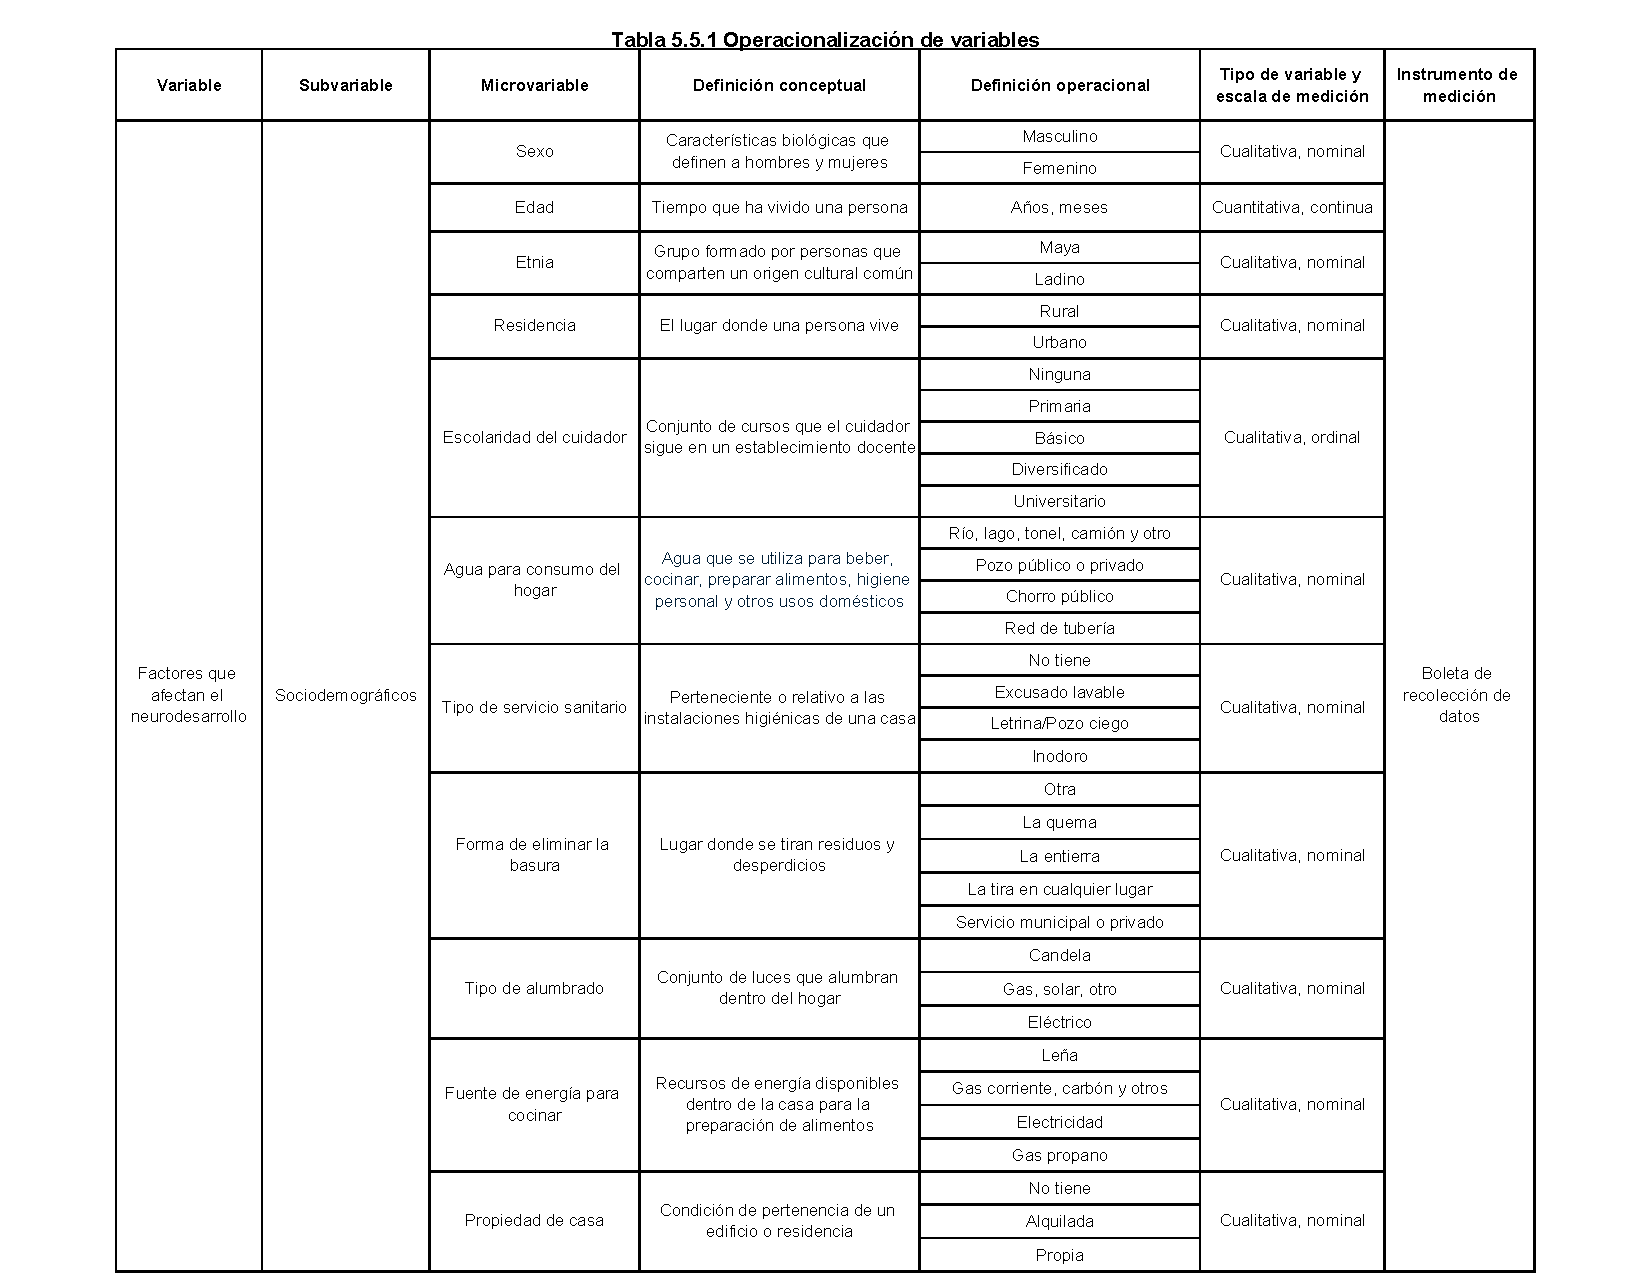
\includepdf[scale=0.90,landscape=true,pages=-,pagecommand={\thispagestyle{plain}}]{OpVariables.pdf}

\section{Hipótesis}
	\begin{enumerate}
		\item Hipótesis nula (H0): No existe una asociación significativa entre
		factores sociodemográficos, condiciones económicas, interacción
		familiar, exposición a dispositivos electrónicos, antecedentes médicos
		perinatales y postnatales, y el riesgo en el neurodesarrollo de niños
		menores de 5 años en servicios de atención primaria de Quetzaltenango.
		\item Hipótesis alternativa (H1): Existe una asociación significativa
		entre factores sociodemográficos, condiciones económicas, interacción
		familiar, exposición a dispositivos electrónicos, antecedentes médicos
		perinatales y postnatales, y el riesgo en el neurodesarrollo de niños
		menores de 5 años en servicios de atención primaria de Quetzaltenango.
	\end{enumerate}

\section{Técnicas de recolección de información e instrumentos de medición}
	\begin{enumerate}
		\item Técnicas de recolección de información: Para llevar a cabo este
		estudio de cohorte prospectivo, se implementarán las siguientes fases:
	\begin{enumerate}
		\item Fase preliminar (Febrero de 2025):
		Se obtuvieron los permisos correspondientes a las autoridades de salud
		del departamento de Quetzaltenango para acceder a los servicios de
		atención primaria seleccionados. Se determinaron estrategias para
		garantizar la uniformidad en la recolección de los datos entre los
		investigadores.
		\item Fase de recolección de datos:
		Se identificarán y reclutarán niños menores de 5 años que cumplan con
		los criterios de inclusión en los servicios de atención primaria
		participantes. Tras obtener el consentimiento informado de los padres o
		tutores, se realizará:
			\begin{itemize}
			\item Evaluación basal del neurodesarrollo mediante la aplicación
			del \asq, seleccionando la versión específica según la edad del
			niño.
			\item Aplicación de un cuestionario estructurado para recolectar
			información sobre factores potencialmente asociados al
			neurodesarrollo.
			\end{itemize}
		\item Fase de clasificación y análisis:
		Los resultados de cada niño serán evaluados conforme al
		puntaje obtenido en el \asq\
		y clasificados en tres categorías:
			\begin{itemize}
			\item Desarrollo típico: puntaje en el área blanca, indicativo de
			un desarrollo acorde a su edad.
			\item Requiere monitoreo: puntaje en el área gris, señalando
			habilidades ligeramente por debajo del promedio.
			\item Retraso en el desarrollo: puntaje en el área negra,
			sugiriendo la necesidad de intervención especializada.
			\end{itemize}
		Se analizarán las asociaciones entre los factores de exposición
		identificados y los resultados de neurodesarrollo en la evaluación.
	\end{enumerate}
	\item Instrumentos de recolección de información
	Para este estudio de cohorte prospectivo, se emplearán los siguientes
	instrumentos:
		\begin{itemize}
		\item \asq: Adaptado al idioma español y ajustado por edad. Esta
		herramienta validada de tamizaje del desarrollo identifica riesgos de
		problemas de neurodesarrollo en niños de 2 a 66 meses. Será aplicado
		por los investigadores con información proporcionada por los padres o
		tutores y mediante observación directa de actividades específicas.
		El \asq\ evalúa cinco áreas del desarrollo: comunicación, motricidad
		gruesa, motricidad fina, resolución de problemas, habilidades
		socioindividuales.

		\item Cuestionario de factores de exposición: Instrumento estructurado
		diseñado específicamente para este estudio que recopilará información
		sobre:
				\begin{itemize}
					\item Variables sociodemográficas (edad, sexo, etnia, nivel
					educativo de los padres)
					\item Variables económicas (empleo de los padres, acceso a
					seguridad social)
					\item Variables de interacción familiar (tiempo de juego,
					disponibilidad de juguetes)
					\item Variables médicas (prematuridad, peso al nacer, tipo
					de parto, lactancia, estado nutricional, etc.)
				\end{itemize}
		\end{itemize}
\end{enumerate}

\section{Plan de análisis de datos}
\begin{enumerate}
	\item Preparación de los datos: Los datos en formato físico serán
	digitados para su uso en el software estadístico Rstudio y python con los
	paquetes numpy y pandas. Se realizará una limpieza de los datos para
	identificar y corregir posibles errores de entrada. Los puntajes obtenidos
	en cada área del desarrollo del \asq\ se convertirán a valores
	estadísticos. 
	
	\item Análisis descriptivo de datos de la cohorte completa: Se calcularán
	frecuencias y porcentajes de los diferentes factores de riesgo presentes en
	la población a estudiar. Se calcularán medidas de tendencia central como
	media, mediana, y desviación estándar de los puntajes del neurodesarrollo.

	\item Análisis comparativo de los resultados del \asq\ de la cohorte
	completa utilizando las siguientes herramientas estadísticas:
		\begin{itemize}
		\item Chi-cuadrado: para determinar si hay asociación significativa
		entre las variables categóricas y riesgo del retraso en el
		neurodesarrollo, se utilizará para evaluar factores de riesgo
		individuales y comparar con desarrollo normal versus desarrollo en
		riesgo.
		\item Análisis de variancia (ANOVA): para comparar medias de puntajes
		del neurodesarrollo en más de dos grupos diferentes de una misma
		categoría y determinar su variación, por ejemplo para evaluar el riesgo
		del neurodesarrollo en valores Z y medidas de tendencia central con
		el grado de escolaridad de los padres de los niños: ninguna, primaria,
		básico, diversificado, universitario.
		\end{itemize}

	\item Análisis de asociación de los resultados del \asq\ del grupo
	estudiado utilizando:
		\begin{itemize}
		\item Odds ratio (OR): para comparar las probabilidades de que se
		presente riesgo en el neurodesarrollo entre dos grupos diferentes.
		Por ejemplo para comparar si los niños con padres que tienen un trabajo
		formal o informal tienen mayor probabilidad o no, de presentar riesgo
		en el neurodesarrollo.
		\end{itemize}
	\item Presentación de resultados: se elaborarán tablas y gráficos
	apropiados con intervalos utilizando el software Rstudio y paquetes de
	CRAN como ggplot2 para análisis y creación de datos informativos.
\end{enumerate}

\section{Principios éticos en la investigación}
Esta investigación se adherirá a los principios éticos clave, tales como:
\begin{itemize}
	\item Consentimiento informado: explicando claramente los objetivos del
	estudio a los padres o tutores y obteniendo su autorización.

	\item Confidencialidad: los datos se mantendrán anónimos y se utilizarán 
	exclusivamente para fines de investigación.

	\item Beneficencia y no maleficencia: buscando maximizar beneficios
	potenciales sin causar daños a los participantes.

	\item El \asq\ es una herramienta validada, respaldada por evidencia
	científica y recomendada por instituciones como UNICEF para su uso en
	evaluación del neurodesarrollo infantil en servicios de atención de
	salud. \cite{UNICEFrespaldo}
\end{itemize}

\printbibliography
\end{document}
